\documentclass[class=beamer,10pt,crop=false]{standalone}
\setbeamersize{text margin left=5mm,text margin right=5mm} 

% Linespacing
\linespread{1.5}

% Font choice
\usepackage{lmodern}

% Use IEEE bibliography style
\bibliographystyle{IEEEtran}

% Ensure UTF8 encoding
\usepackage[utf8]{inputenc}

% Language standard (not too important)
\usepackage[english]{babel}

% Math
\usepackage{amsmath}

% Colour
\usepackage{color}
% \usepackage[usenames,dvipsnames]{xcolor}

% Hyperlinks & References
\usepackage{hyperref}
\definecolor{linkColour}{RGB}{77,71,179}
\hypersetup{
    colorlinks=true,
    linkcolor=linkColour,
    filecolor=linkColour,
    urlcolor=linkColour,
    citecolor=linkColour,
}
\urlstyle{same}

% Automatically correct front-side quotes
\usepackage[autostyle=false, style=ukenglish]{csquotes}
\MakeOuterQuote{"}

% Graphics
\usepackage{graphicx}
\graphicspath{{Images/}{../Images/}{../../Images/}}
\usepackage{makecell}
\usepackage{transparent}

% SI units
\usepackage{siunitx}

% Microtype goodness
\usepackage{microtype}

% Listings
\usepackage[T1]{fontenc}
\usepackage{listings}
\usepackage[scaled=0.8]{DejaVuSansMono}

\definecolor{backgroundColour}{RGB}{250,250,250}
\definecolor{commentColour}{RGB}{73, 175, 102}
\definecolor{identifierColour}{RGB}{196, 19, 66}
\definecolor{stringColour}{RGB}{252, 156, 30}
\definecolor{keywordColour}{RGB}{50, 38, 224}
\definecolor{lineNumbersColour}{RGB}{127,127,127}
\lstset{
  language=Matlab,
  captionpos=b,
  aboveskip=0pt,belowskip=0pt,
  backgroundcolor=\color{backgroundColour},
  basicstyle=\footnotesize,        % the size of the fonts that are used for the code
  breakatwhitespace=false,         % sets if automatic breaks should only happen at whitespace
  breaklines=true,                 % sets automatic line breaking
  postbreak=\mbox{\textcolor{red}{$\hookrightarrow$}\space},
  commentstyle=\color{commentColour},    % comment style
  identifierstyle=\color{identifierColour},
  stringstyle=\color{stringColour},
   keywordstyle=\color{keywordColour},       % keyword style
  %escapeinside={\%*}{*)},          % if you want to add LaTeX within your code
  extendedchars=true,              % lets you use non-ASCII characters; for 8-bits encodings only, does not work with UTF-8
  frame=single,	                   % adds a frame around the code
  keepspaces=true,                 % keeps spaces in text, useful for keeping indentation of code (possibly needs columns=flexible)
  morekeywords={*,...},            % if you want to add more keywords to the set
  numbers=left,                    % where to put the line-numbers; possible values are (none, left, right)
  numbersep=5pt,                   % how far the line-numbers are from the code
  numberstyle=\tiny\color{lineNumbersColour}, % the style that is used for the line-numbers
  rulecolor=\color{black},         % if not set, the frame-color may be changed on line-breaks within not-black text (e.g. comments (green here))
  showspaces=false,                % show spaces everywhere adding particular underscores; it overrides 'showstringspaces'
  showstringspaces=false,          % underline spaces within strings only
  showtabs=false,                  % show tabs within strings adding particular underscores
  stepnumber=1,                    % the step between two line-numbers. If it's 1, each line will be numbered
  tabsize=2,	                   % sets default tabsize to 2 spaces
  %title=\lstname                   % show the filename of files included with \lstinputlisting; also try caption instead of title
}

% Caption stuff
\usepackage[hypcap=true, justification=centering]{caption}
\usepackage{subcaption}

% Glossary package
% \usepackage[acronym]{glossaries}
\usepackage{glossaries-extra}
\setabbreviationstyle[acronym]{long-short}

% For Proofs & Theorems
\usepackage{amsthm}

% Maths symbols
\usepackage{amssymb}
\usepackage{mathrsfs}
\usepackage{mathtools}

% For algorithms
\usepackage[]{algorithm2e}

% % Add section content
% \AtBeginSection[]
% {
%     \begin{frame}
%         \frametitle{Outline}
%         \tableofcontents[currentsection]
%     \end{frame}
% }

\begin{document} 

\section{Digital Audio Broadcasting: Processing Chain Design}

\subsection{Overview}
\begin{frame}
    \label{slide:dab-proc_overview}
    \frametitle{\subsecname}
    
    \begin{figure}[htbp]
        \centering
        \captionsetup{type=figure}
        \def\svgwidth{\linewidth}
        {\linespread{0.8}
        \tiny
        \input{../Images/Pres_BD_Overview_All.pdf_tex}}
        \caption{Block diagram showing entire DAB processing chain}
        \label{fig:BD_Overview_All}
    \end{figure}
    
\end{frame}


\subsection{Pre-processing}
\begin{frame}
    \label{slide:dab-proc_preprocess}
    \frametitle{\subsecname}
    
    \begin{figure}[htbp]
        \centering
        \captionsetup{type=figure}
        \def\svgwidth{\linewidth}
        {\linespread{0.8}
            \scriptsize
            \input{../Images/Pres_BD_Preprocess_All.pdf_tex}}
        \caption{Block diagram showing pre-processing block}
        \label{fig:BD_Preprocess_All}
      \end{figure}
      
\end{frame}

% \subsubsection{Frame Synchronisation via PRS detection}
% \begin{frame}
%     \label{slide:dab-proc_prs-detect}
%     \frametitle{\subsubsecname}
    
      
% \end{frame}


\subsection{Demodulation}
\begin{frame}
    \label{slide:dab-proc_demod}
    \frametitle{\subsecname}
    
    \begin{figure}[htbp]
        \centering
        \captionsetup{type=figure}
        \def\svgwidth{\linewidth}
        {\linespread{0.8}
            \scriptsize
            \input{../Images/Pres_BD_Demod_All.pdf_tex}}
        \caption{Block diagram showing demodulation block}
        \label{fig:BD_Demod_All}
      \end{figure}
      
\end{frame}

\subsubsection{Symbols Unpacking}
\begin{frame}
    \label{slide:dab-proc_symbols-unpack}
    \frametitle{\subsecname : \subsubsecname}
    
    \begin{figure}[htbp]
        \centering
        \captionsetup{type=figure}
        \def\svgwidth{\linewidth}
        {\linespread{0.8}
            \scriptsize
            \input{../../Images/symbols_unpack.pdf_tex}}
        \caption{Graphical summary of \texttt{symbols\_unpack} function}
        \label{fig:symbols_unpack}
      \end{figure}
      
\end{frame}

\subsubsection{OFDM Demultiplexing}
% \begin{frame}[fragile]
%     \frametitle{\subsecname : \subsubsecname}

%     Use FFT for demultiplexing OFDM symbols.

%     \begin{figure}[htbp]
%         \centering
%         \captionsetup{type=figure}
%         \def\svgwidth{\linewidth}
%         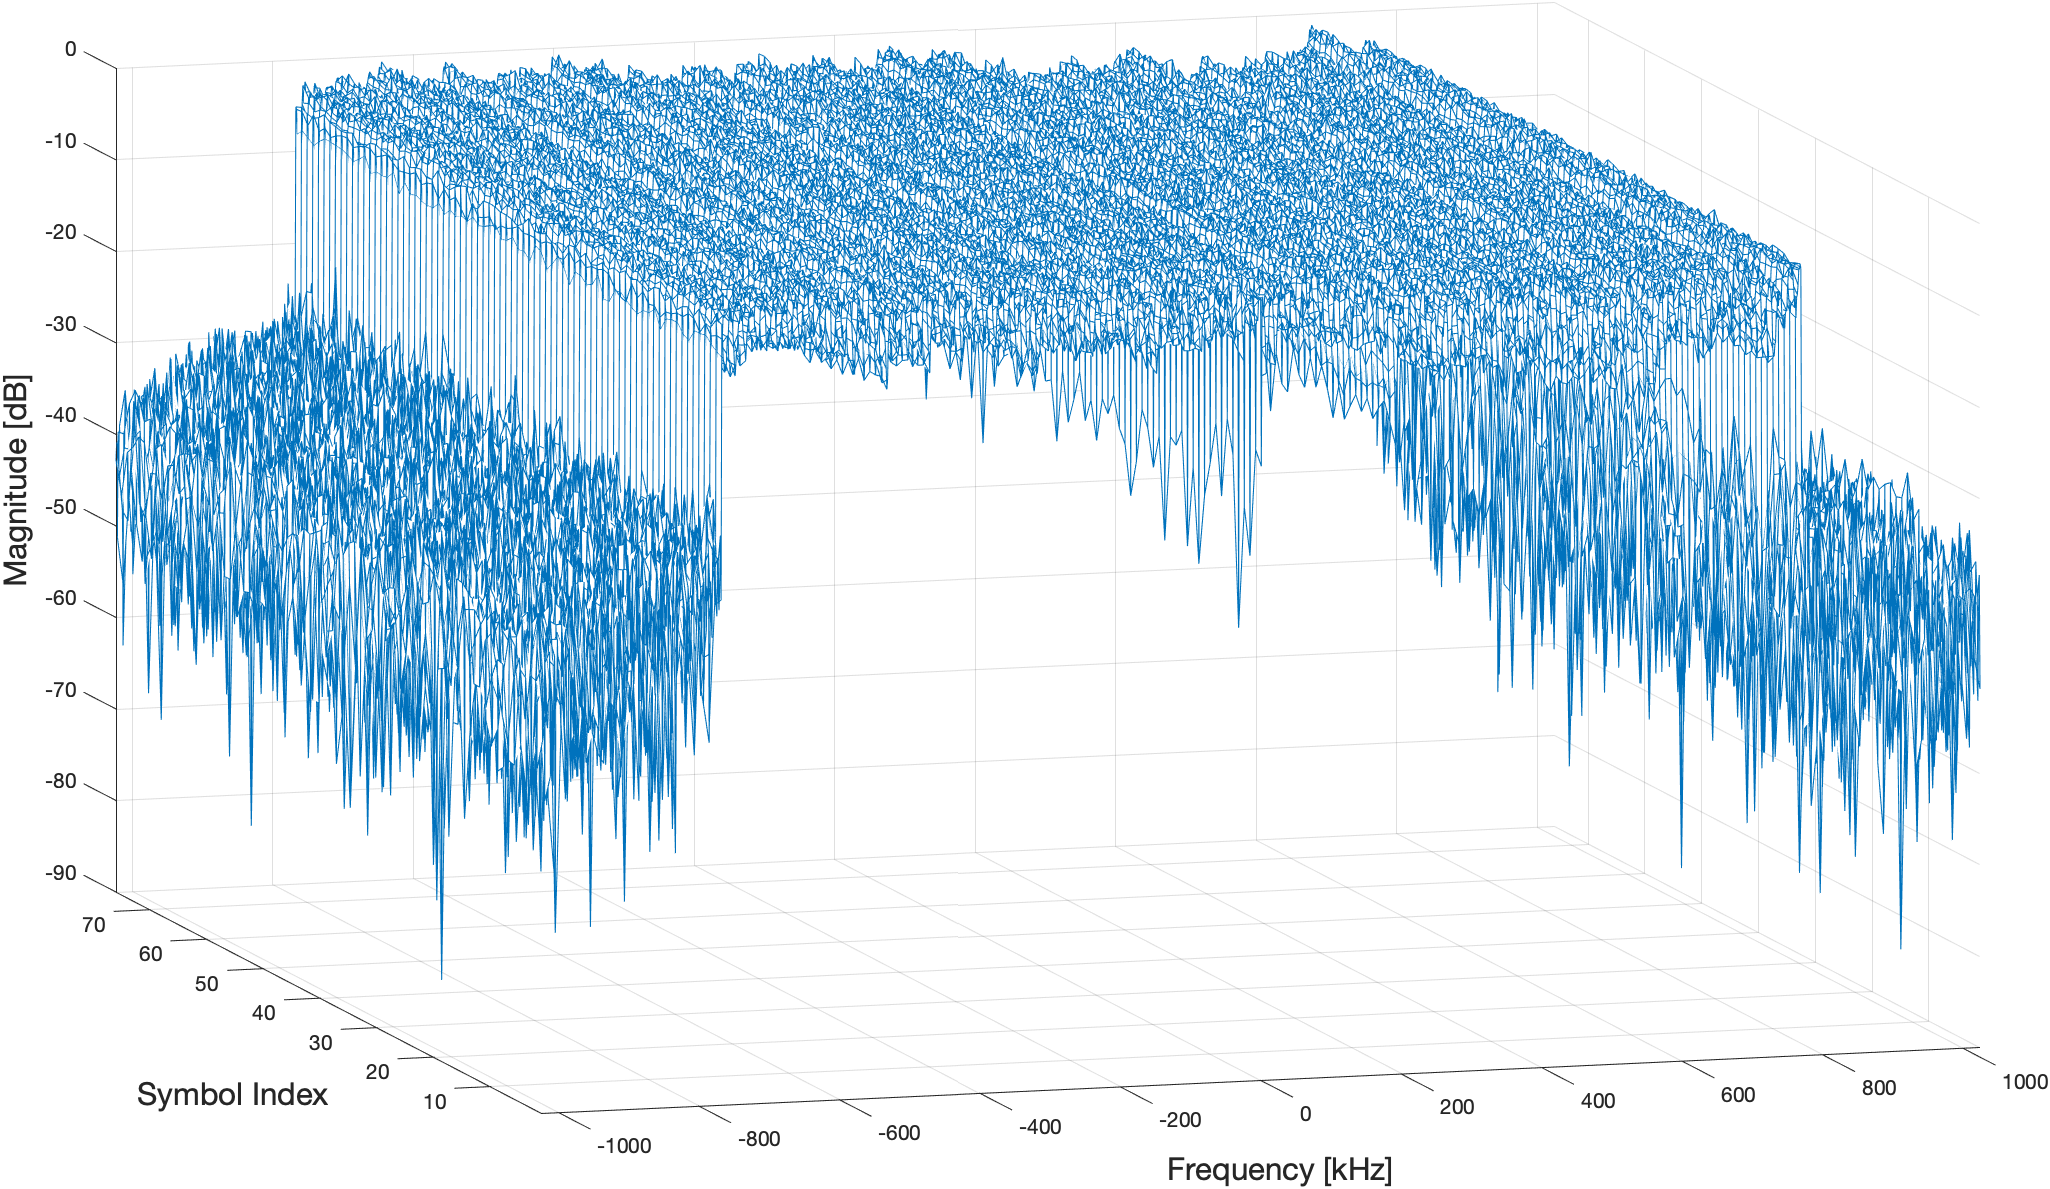
\includegraphics[width=0.6\linewidth]{../Images/plots/ofdm-surface-raw.png}
%         \caption{Surface plot of a DAB frame's OFDM symbols}
%         \label{fig:ofdm-surface}
%       \end{figure}
      
% \end{frame}

\begin{frame}
    \label{slide:dab-proc_ofdm-demux}
    \frametitle{\subsecname : \subsubsecname}
    
    \begin{figure}[htbp]
        \centering
        \captionsetup{type=figure}
        \def\svgwidth{\linewidth}
        {\linespread{0.8}
            \scriptsize
            \input{../../Images/ofdm_demux.pdf_tex}}
        \caption{Graphical summary of \texttt{ofdm\_demux} function}
        \label{fig:ofdm_demux}
      \end{figure}
      
\end{frame}

\subsubsection{DQPSK Demapping}
\begin{frame}
    \label{slide:dab-proc_dqpsk-demap}
    \frametitle{\subsecname : \subsubsecname}
    
    \begin{figure}[htbp]
        \centering
        \captionsetup{type=figure}
        \def\svgwidth{\linewidth}
        {\linespread{0.8}
            \scriptsize
            \input{../../Images/dqpsk_demap.pdf_tex}}
        \caption{Graphical summary of \texttt{dqpsk\_demap} function}
        \label{fig:dqpsk_demap}
      \end{figure}
      
\end{frame}


\subsubsection{Frequency Deinterleaving}
\begin{frame}
    \label{slide:dab-proc_freq-deinterleave}
    \frametitle{\subsecname : \subsubsecname}
    
    \begin{figure}[htbp]
        \centering
        \captionsetup{type=figure}
        \def\svgwidth{\linewidth}
        {\linespread{0.8}
            \scriptsize
            \input{../../Images/freq_deinterleave.pdf_tex}}
        \caption{Graphical summary of \texttt{freq\_deinterleave} function}
        \label{fig:freq_deinterleave}
      \end{figure}
      
\end{frame}

\subsubsection{DQPSK Snapping}
% \begin{frame}
%     \frametitle{\subsecname : \subsubsecname}
    
%     \begin{figure}[htbp]
%         \centering
%         \captionsetup{type=figure}
%         \def\svgwidth{\linewidth}
%         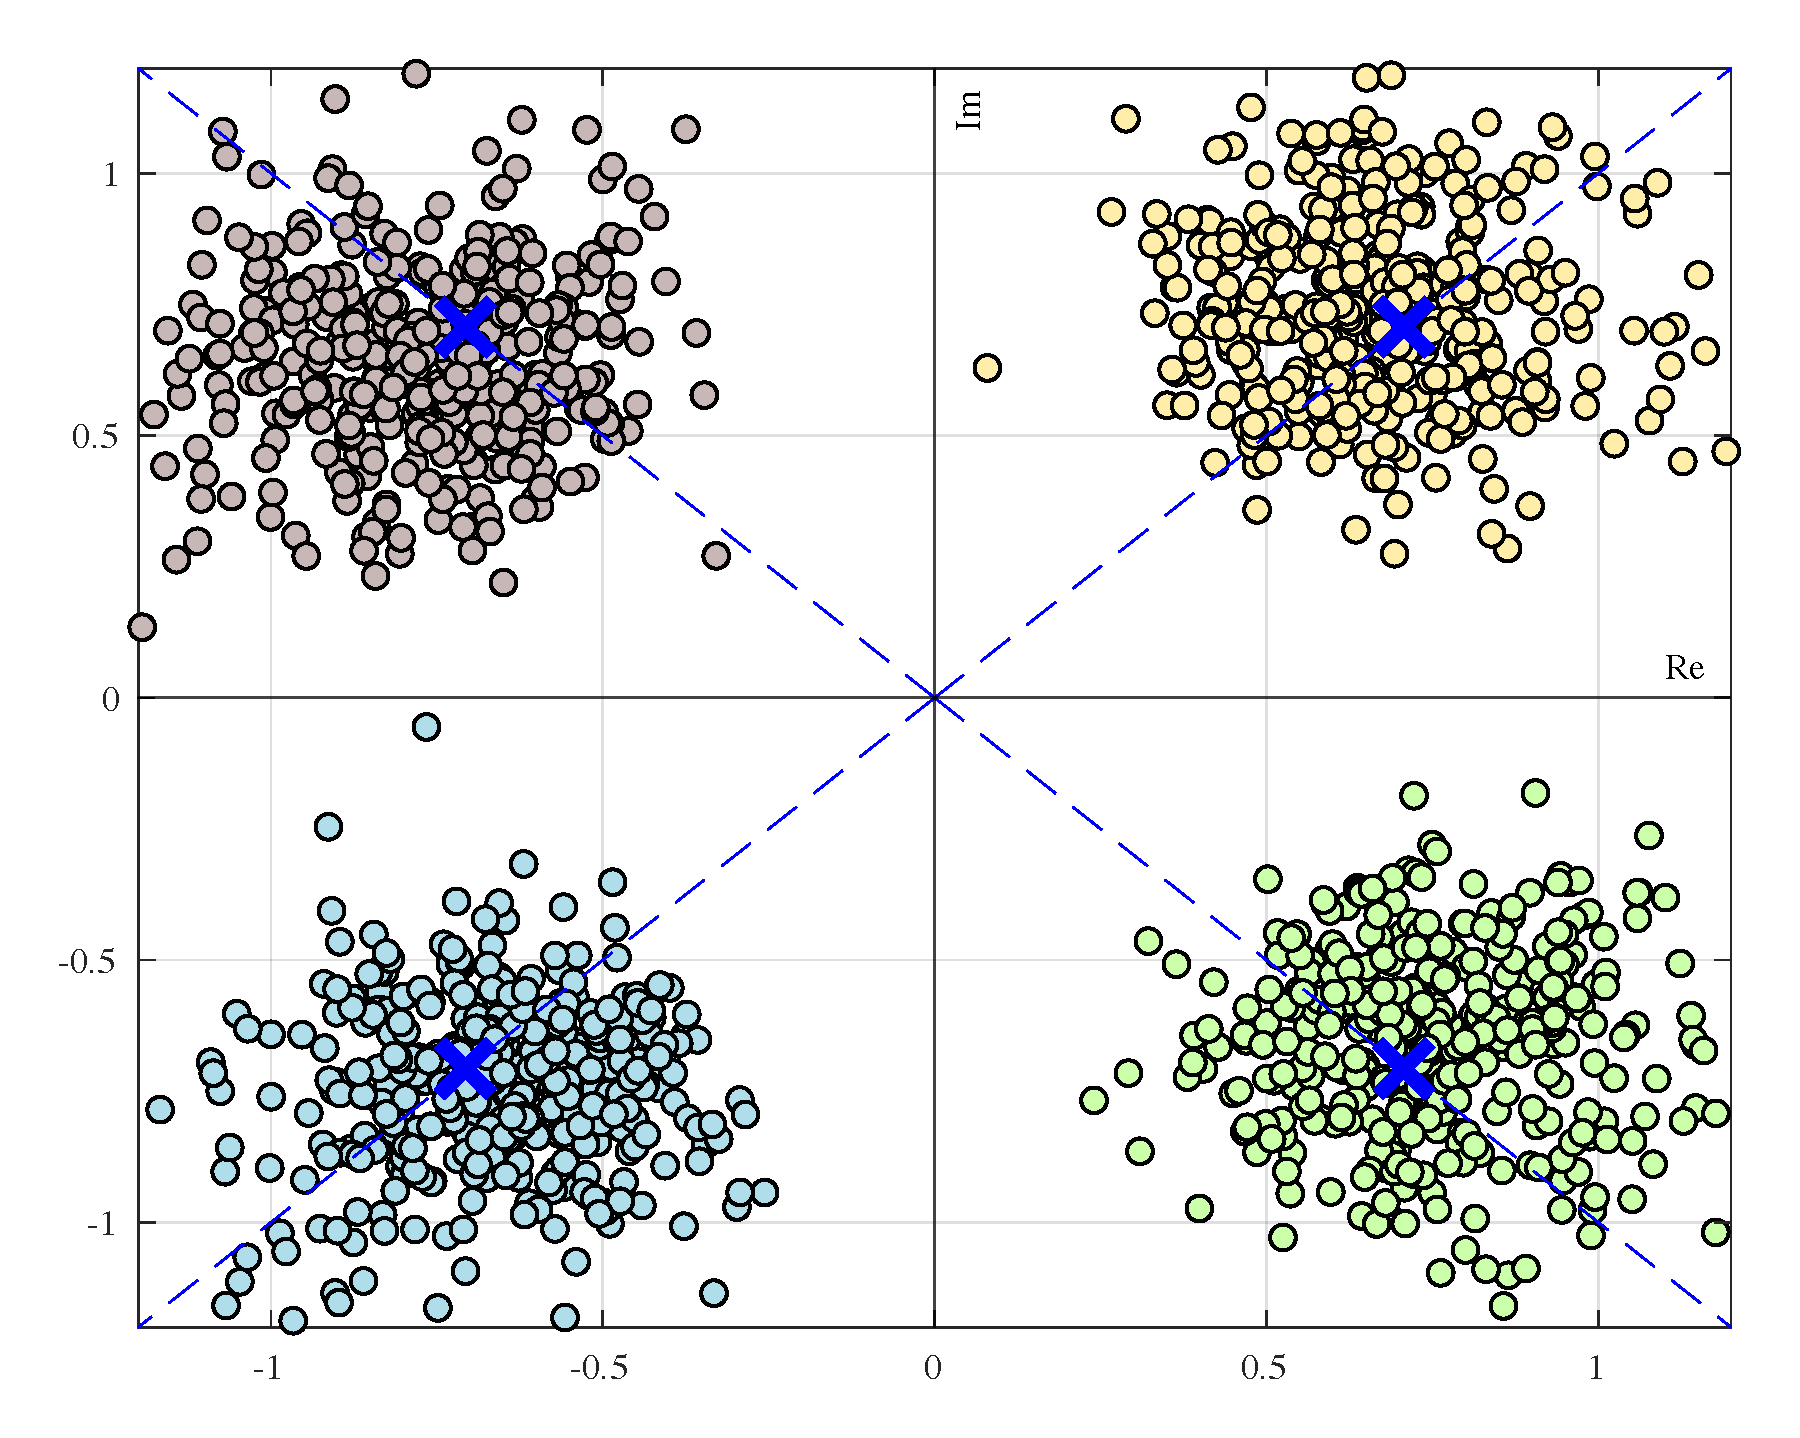
\includegraphics[width=0.6\textwidth]{../Images/dqpsk_snap-rtl.pdf}
%         \caption{Depiction of the DQPSK snapping functionality}
%         \label{fig:dqpsk_snap-rtl}
%       \end{figure}
      
% \end{frame}

\begin{frame}
    \label{slide:dab-proc_dqpsk-snap}
    \frametitle{\subsecname : \subsubsecname}
    
    \begin{figure}[htbp]
        \centering
        \captionsetup{type=figure}
        \def\svgwidth{\linewidth}
        {\linespread{0.8}
            \scriptsize
            \input{../../Images/dqpsk_snap.pdf_tex}}
        \caption{Graphical summary of \texttt{dqpsk\_snap} function}
        \label{fig:dqpsk_snap}
      \end{figure}
      
\end{frame}
    
\subsubsection{Error Correction}
\begin{frame}
    \label{slide:dab-proc_error-correct}
    \frametitle{\subsecname : \subsubsecname}
        
    Not completed due to the scope of this project; nevertheless, an important part of a demodulation-remodulation chain.
        
\end{frame}

%%%%%%%%%%%%%%%%%%%%%%%%%%%%%%%%%%%%%%%%%%%%%%%%%%%%%%%%%%%%%%%
% REMODULATION
%%%%%%%%%%%%%%%%%%%%%%%%%%%%%%%%%%%%%%%%%%%%%%%%%%%%%%%%%%%%%%%

\subsection{Remodulation}
\begin{frame}
    \label{slide:dab-proc_remod}
    \frametitle{\subsecname}
    
    \begin{figure}[htbp]
        \centering
        \captionsetup{type=figure}
        \def\svgwidth{\linewidth}
        {\linespread{0.8}
            \scriptsize
            \input{../Images/Prers_BD_Remod_All.pdf_tex}}
        \caption{Block diagram showing remodulation block}
        \label{fig:BD_Demod_All}
      \end{figure}
      
\end{frame}

\subsubsection{Frequency Interleaving}
\begin{frame}
    \label{slide:dab-proc_freq-interleave}
    \frametitle{\subsecname : \subsubsecname}
    
    \begin{figure}[htbp]
        \centering
        \captionsetup{type=figure}
        \def\svgwidth{\linewidth}
        {\linespread{0.8}
            \scriptsize
            \input{../../Images/freq_interleave.pdf_tex}}
        \caption{Graphical summary of \texttt{freq\_interleave} function}
        \label{fig:freq_interleave}
      \end{figure}
      
\end{frame}

\subsubsection{DQPSK Mapping}
\begin{frame}
    \label{slide:dab-proc_dqpsk-map}
    \frametitle{\subsecname : \subsubsecname}
    
    \begin{figure}[htbp]
        \centering
        \captionsetup{type=figure}
        \def\svgwidth{0.9\linewidth}
        {\linespread{0.8}
            \scriptsize
            \input{../../Images/dqpsk_map.pdf_tex}}
        \caption{Graphical summary of \texttt{dqpsk\_map} function}
        \label{fig:dqpsk_map}
      \end{figure}
      
\end{frame}

\subsubsection{OFDM Multiplexing}
\begin{frame}
    \label{slide:dab-proc_ofdm-mux}
    \frametitle{\subsecname : \subsubsecname}
    
    \begin{figure}[htbp]
        \centering
        \captionsetup{type=figure}
        \def\svgwidth{\linewidth}
        {\linespread{0.8}
            \scriptsize
            \input{../../Images/ofdm_mux.pdf_tex}}
        \caption{Graphical summary of \texttt{ofdm\_mux} function}
        \label{fig:ofdm_mux}
      \end{figure}
      
\end{frame}

\subsubsection{Symbols Packing}
\begin{frame}
    \label{slide:dab-proc_symbols-pack}
    \frametitle{\subsecname : \subsubsecname}
    
    \begin{figure}[htbp]
        \centering
        \captionsetup{type=figure}
        \def\svgwidth{\linewidth}
        {\linespread{0.8}
            \scriptsize
            \input{../../Images/symbols_pack.pdf_tex}}
        \caption{Graphical summary of \texttt{symbols\_pack} function}
        \label{fig:symbols_pack}
      \end{figure}
      
\end{frame}

\end{document}